\documentclass[]{beamer}


%%%%%%%%%%%%%%%%%%%%%%%%%%%%%%%%%%%%%
%% Select input file encoding:
%%   utf8   - UTF-8, nowadays standard on most operating sytems
%%   latin1 - ISO-8859-1
\usepackage[utf8]{inputenc}                 

%%%%%%%%%%%%%%%%%%%%%%%%%%%%%%%%%%%%%
%% Select language
%%
%\usepackage[ngerman]{babel}        % Deutsch, neue Rechtschreibung
\usepackage[english]{babel}         % English



\usetheme{rwth}

\usepackage[T1]{fontenc}                        % Font encoding (don't change!)
\usepackage{lmodern}                            % Select Linux Modern Fonts (don't change)
\usepackage{graphicx}                           % needed to include graphics (don't change)

%%%%%%%%%%%%%%%%%%%%%%%%%%%%%%%%%%%%%
%% import packages for content
%%
\usepackage{listings}                           % for lstlisting and \lstinline|..|
%% TikZ can be used to /program/ graphics.
\usepackage{tikz}                                % comment-out, if you don't need this.
%% some TikZ-libraries and settings for the examples...
%\usetikzlibrary{shapes,arrows}                  
\usetikzlibrary{shadings}           % GW: color gradients
\usetikzlibrary{calc,positioning,fit,matrix,shadows,chains,arrows,shapes,spy,fadings}
%\usepackage{pgfplots}
%\usetikzlibrary{pgfplots.units,shapes.symbols,shapes.arrows}
%\usetikzlibrary{pgfplots.external}
%\tikzexternalize[prefix=tmp/]



%%%%%%%%%%%%%%%%%%%%%%%%%%%%%%%%%%%%%
%% configure title page and author information
%%-------------------------------
%% You can always provide a short version: \title[short]{long title}
%%   title        -- Title of the presentation
%%                   The title appears on the first page and may contain a line break: \\ 
%%                   The short title appears in the footer line
%%   subtitle     -- Appears below the title
%%   titlegraphic -- Currently not supported
%%   author       -- Name of the author(s)
%%   email        -- E-Mail address of author (optional)
%%   institute    -- Name of the institution (e.g. chair)
%%   webaddress   -- Web address (default is www.rwth-aachen.de), displayed on last slide
%%   date         -- Date of the presentation (or use \date to insert the date of the PDF generation)
%%   subject      -- This is only for the PDF meta data
%%   keywords     -- This is only for the PDF meta data
%%   logo         -- Logo, don't change (given by coporate identity templates)
%%   instlogo     -- Logo of institute/chair, if given: will be shown in foot line
\title[LLVM: Code generation + autovec]{Code Generation and Autovectorization\\ with LLVM}
\subtitle{Seminar Automation, Compilers, and Code-Generation}
%\titlegraphic{}            
\author{Simon Grätzer}
\email{simon.graetzer@rwth-aachen.de}                          % optionally
\institute{High-Performance and Automatic Computing}
\webaddress{http://graetzer.org/}                        % overrides www.rwth-aachen.de
\date{06.07.2016}
\subject{LLVM: Code generation + Autovectorization}          
\keywords{LLVM, Code Generation, Autovec}
\instlogo{
\includegraphics[height=8mm]{logos/hpac}}        % optionally

% supress error because of inkscape bug
\pdfsuppresswarningpagegroup=1

\begin{document}

%%
%% the title slide is generated automatically (at begin document)
%%

%%
%% Use \section{} to divide your presentation into chapters.
%% Each \section{} generates a section frame automatically.
%% The variant \section*{} will not appear in the table of contents and will not generate a section frame
%%
\section*{Introduction}
\begin{frame}{Introduction}
  \begin{itemize}
    \item Code Generation Process in LLVM
    \begin{itemize}
      \item The frontend of LLVM outputs target independent LLVM IR code
      \item Compiler Backend has to transform this into machine code for a specific platform
      \item In this process it can apply optimizations for the targeted platform
    \end{itemize}
    \item Auto-Vectorization in LLVM
    \begin{itemize}
      \item Converts code using only scalar data types and operations into code using vector-types and operations.
      \item Vectorizing can lead to significant performance gains.
      \item The compiler can perform vectorizing for the programmer (sometimes).
    \end{itemize}
  \end{itemize}
\end{frame}

%%
%% Table of contents (automatically collects all \section{} and \subsection{} entries).
%% (run pdflatex multiple times to get all cross references correct)
%%
\begin{frame}{Agenda}
  \tableofcontents
\end{frame}

\section{Code Generation}

\begin{frame}{Overview}
  \begin{itemize}
    \item Code generation is one of the most complex tasks in the LLVM
    \item We need to "lower" the LLVM IR into the corresponding machine code
    \item Optimize code and replace unsupported data types and operations for the target platform
    \item LLVM supports this process through it's \textbf{target-independent code generator} framework
    \item This presentation focuses on this framework
  \end{itemize}
\end{frame}

\begin{frame}{Processing Steps}
  \begin{enumerate}
    \item Instruction Selection
    \item Scheduling and Formation
    \item SSA-based Machine Code Optimizations
    \item Register Allocation
    \item Prolog/Epilog Code Insertion
    \item Final Optimizations
    \item Code Emission
  \end{enumerate}
\end{frame}

%\subsection{Instruction Selection}

%%%%%%%%%%%%%%%%%%%%%%%%%%%%%%%%%%%%%%%%%%%%%%%%%%%%%%%%%%%%%%%%%%%%%%%%%
\begin{frame}[fragile]{Reminder: LLVM IR}
  \vfill
  Let's consider a simple C function:
  \begin{lstlisting}[language=C,gobble=4]
    int foo(int aa, int bb, int cc) {
      int sum = aa + bb;
      return sum / cc;
    }
  \end{lstlisting}
  \vfill
\end{frame}


%%%%%%%%%%%%%%%%%%%%%%%%%%%%%%%%%%%%%%%%%%%%%%%%%%%%%%%%%%%%%%%%%%%%%%%%%
\begin{frame}[fragile]{Reminder: LLVM IR}
  \vfill
  Is transforms into the LLVM IR: \lstinline[language=bash]{clang -cc1 foo.c -emit-llvm}\\
  \begin{lstlisting}[language=LLVM,gobble=4]
    define i32 @foo(i32 %aa, i32 %bb, i32 %cc) {
      entry:
        %add = add nsw i32 %aa, %bb
        %div = sdiv i32 %add, %cc
        ret i32 %div
      }
  \end{lstlisting}
  \vfill
  Note: This is still a very high level code representation. Variables are uniquely named and 
  assigned exactly once this is called static single assignment (SSA) form.
\end{frame}

%%%%%%%%%%%%%%%%%%%%%%%%%%%%%%%%%%%%%%%%%%%%%%%%%%%%%%%%%%%%%%%%%%%%%%%%%
\begin{frame}{Directed Acyclic Graph}
  DAG's represent the program code as basic blocks:
  \begin{columns}[b]
    \begin{column}{.5\textwidth}
    \begin{center}
      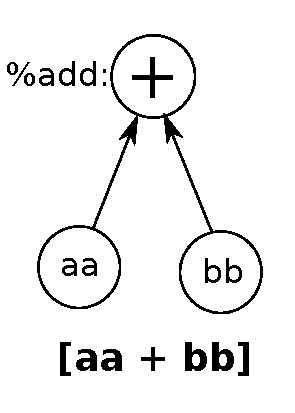
\includegraphics[width=.5\textwidth]{pictures/dag_step_1}
    \end{center}
    \end{column}
    \begin{column}{.5\textwidth}
      \begin{center}
      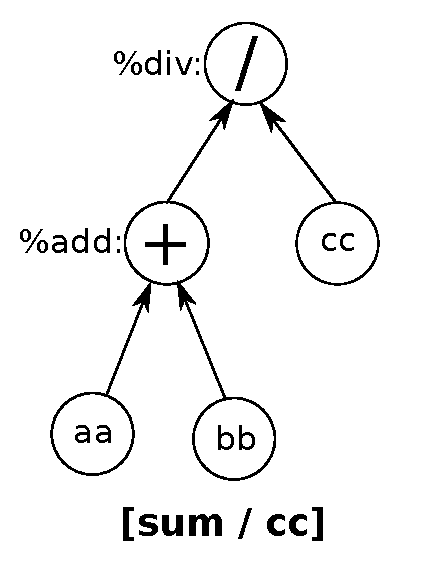
\includegraphics[width=.65\textwidth]{pictures/dag_step_2}
      \end{center}
    \end{column}
  \end{columns}
  \begin{enumerate}
    \item Leaf nodes represent identifiers, names or constants.
    \item Interior nodes can represent operators.
    \item Interior nodes also represent results of expressions or identifiers of locations where values are to be stored.
  \end{enumerate}
\end{frame}

%%%%%%%%%%%%%%%%%%%%%%%%%%%%%%%%%%%%%%%%%%%%%%%%%%%%%%%%%%%%%%%%%%%%%%%%%
\begin{frame}{SelectionDAG}
  \begin{itemize}
    \item In LLVM the DAG is called a SelectionDAG, based on the \lstinline[language=c++]{SDNode} class.
    \item LLVM defines a series of node types, which represent operators, vars etc.
    \item Works well for many phases of code generation.
    \item It is possible to perform transformations on the SelectionDAG by using techniques like \textbf{pattern matching} 
    \item Transformations are performed in multiple passes on the DAG.
    \item Many performance optimizations are performed directly on this representation (e.g. peephole optimizations)
  \end{itemize}
\end{frame}

%%%%%%%%%%%%%%%%%%%%%%%%%%%%%%%%%%%%%%%%%%%%%%%%%%%%%%%%%%%%%%%%%%%%%%%%%
\begin{frame}[fragile]{SelectionDAG: Example}
  \begin{lstlisting}[language=LLVM,gobble=4]
    define i64 @imul(i64 %a, i64 %b) nounwind readnone {
    entry:
      %mul = mul nsw i64 %b, %a
      ret i64 %mul
    }
  \end{lstlisting}

  \begin{itemize}
    \item This gets expanded into an initial SelectionDAG.
    \item Afterwards the first optimization pass is performed.
  \end{itemize}
\end{frame}

%%%%%%%%%%%%%%%%%%%%%%%%%%%%%%%%%%%%%%%%%%%%%%%%%%%%%%%%%%%%%%%%%%%%%%%%%
\begin{frame}{SelectionDAG: Example}
  \begin{center}
  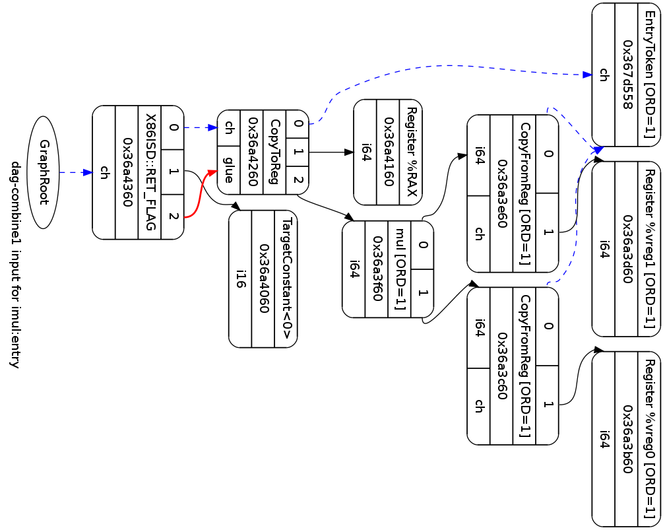
\includegraphics[width=.8\textwidth]{pictures/sdag_mul}
  \end{center}
\end{frame}

%%%%%%%%%%%%%%%%%%%%%%%%%%%%%%%%%%%%%%%%%%%%%%%%%%%%%%%%%%%%%%%%%%%%%%%%%
\begin{frame}{Legalize Types Phase}
\begin{itemize}
    \item The current SelectionDAG is considered \textit{illegal}, because not all types might be supported
          by the target platform.
    \item For example a target might require that all single floating point values are promoted to doubles
          or that bytes/shorts are handled as 32bit integers.
    \item The following operations have to be applied until the DAG is \textit{legal}:
          \begin{itemize}
            \item Promoting: Small types are transformed to larger types.
            \item Expanding: Large integer types are broken up into smaller ones.
          \end{itemize}
    \item The same needs to be applied for LLVMs vector types (used for SIMD instructions)
\end{itemize}
\end{frame}

%%%%%%%%%%%%%%%%%%%%%%%%%%%%%%%%%%%%%%%%%%%%%%%%%%%%%%%%%%%%%%%%%%%%%%%%%
\begin{frame}{Legalizes Operations Phase}
\begin{itemize}
  \item Converts a DAG to only use the operations that are natively supported.
  \item Some CPU's have constraints, like not supporting every operation on all data types.\\
        E.g.\ x86 does not support byte conditional moves.
  \item The legalizer has to convert those operations:
  \begin{itemize}
    \item Expansion: Replace the operation within a sequence of supported operations (open-coding)
    \item Promotion: Change a type to a larger type which supports the operation.
 %   \item Custom: Replace an operation with a target specific way of doing something eqviv.
  \end{itemize} 
\end{itemize}
\end{frame}

%%%%%%%%%%%%%%%%%%%%%%%%%%%%%%%%%%%%%%%%%%%%%%%%%%%%%%%%%%%%%%%%%%%%%%%%%
\begin{frame}{Optimization of DAG}
\begin{itemize}
    \item The optimization phase is run three times on the DAG.
    \item First in the beginning on the original DAG:
      \begin{itemize}
        \item Allows the initial code to be cleaned up.
        \item For example allows to perform optimizations which depend on knowledge of the original data types.
      \end{itemize}
    \item Once after both "legalization" phases (introduced later):
      \begin{itemize}
        \item Clean up the potentially messy code generated by these passes, allows them to remain simple.
        \item Optimizes the inserted sign and zero extensions.
      \end{itemize}
  \end{itemize}
\end{frame}

\subsection{Selection Phase}

%%%%%%%%%%%%%%%%%%%%%%%%%%%%%%%%%%%%%%%%%%%%%%%%%%%%%%%%%%%%%%%%%%%%%%%%%
\begin{frame}[fragile]{Generating Machine Instructions}
The SelectionDAG is transformed into another DAG based on the \lstinline[language=c++]{MachineSDNode} class.\\
An instance of \lstinline[language=c++]{MachineSDNode} contains all information 
necessary to generate the machine code instructions.

\begin{block}{Example LLVM IR:}
\begin{lstlisting}[language=LLVM,gobble=4]
  %t1 = fadd float %W, %X
  %t2 = fmul float %t1, %Y
  %t3 = fadd float %t2, %Z
\end{lstlisting}
\end{block}
\end{frame}

%%%%%%%%%%%%%%%%%%%%%%%%%%%%%%%%%%%%%%%%%%%%%%%%%%%%%%%%%%%%%%%%%%%%%%%%%
\begin{frame}[fragile]{Example}

\begin{columns}[T]
  \begin{column}{.6\textwidth}
    The previous IR code would be equivalent to the following DAG:
    \lstinline[language=c++]{(fadd:f32 (fmul:f32 (fadd:f32 W, X), Y), Z)}
  \end{column}
  \begin{column}{.4\textwidth}
    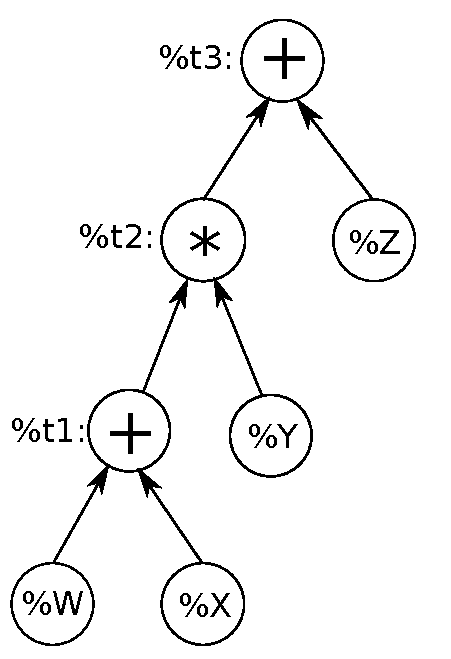
\includegraphics[width=.9\textwidth]{pictures/dag_mul_add}
  \end{column}
\end{columns}

\end{frame}

%%%%%%%%%%%%%%%%%%%%%%%%%%%%%%%%%%%%%%%%%%%%%%%%%%%%%%%%%%%%%%%%%%%%%%%%%
\begin{frame}[fragile]{Example}
If a target supports floating point multiply-and-add (\textbf{FMA}) operations the output can be simplified.
On the PowerPC platform the \textit{FMADDS} operation multiplies the first two parameters and adds the third.\\
Therefore the DAG can be simplified:\\
\lstinline{(FMADDS (FADDS W, X), Y, Z)}
\begin{center}
      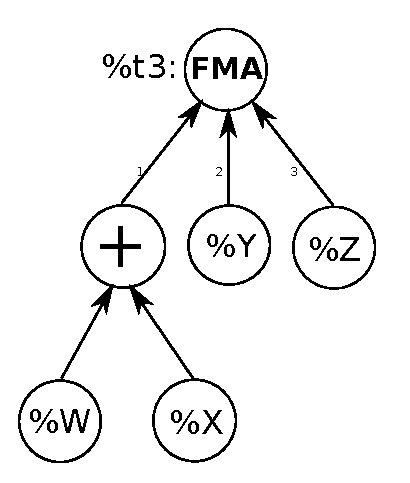
\includegraphics[width=.4\textwidth]{pictures/dag_fma}
\end{center}
\end{frame}

%%%%%%%%%%%%%%%%%%%%%%%%%%%%%%%%%%%%%%%%%%%%%%%%%%%%%%%%%%%%%%%%%%%%%%%%%

\subsection{Scheduling and Formation}
\begin{frame}{}
\begin{itemize}
  \item Takes the \textit{legal} SelectionDAG, which now contains the actual target instructions.
  \item The Scheduler assigns an order to every node which contains an instruction.
  \item There scheduler needs to take the constraints of the machine into account, e.g.\
  \begin{itemize}
    \item Optimize order for minimal register pressure, i.e.\ since the number of registers is limited we want 
          to minimize the number of memory loads or stores (\textit{spills} and \textit{reloads}).
    \item Take instruction latencies into account.
  \end{itemize}
  \item This pass outputs a list of machine instructions, the SelectionDAG is discarded.
\end{itemize}
\end{frame}

%%%%%%%%%%%%%%%%%%%%%%%%%%%%%%%%%%%%%%%%%%%%%%%%%%%%%%%%%%%%%%%%%%%%%%%%%
\subsection{Register Allocation Phase}
\begin{frame}{}

\begin{itemize}
  \item Up until now, we still use an unlimited amount of \textit{virtual registers} in SSA-form.
  \item These need to be mapped to a limited amount of \textit{physical registers}.
  \item When the number of physical registers is not big enough, we need to map some 
        virtual registers into memory. 
  \item These virtual registers are called \textit{spilled virtuals}.
\end{itemize}

\end{frame}

%%%%%%%%%%%%%%%%%%%%%%%%%%%%%%%%%%%%%%%%%%%%%%%%%%%%%%%%%%%%%%%%%%%%%%%%%
\begin{frame}{Live Intervals}

\begin{itemize}
  \item Live Intervals are the intervals where a variable is actually used.
  \item We need to determine if two or more virtual registers are live at the same point and require the same physical register.
  \item In this case one virtual register must be \textit{spilled}.
  \item The register allocator can use this information to determine the registers to spill.
\end{itemize}

\end{frame}

%%%%%%%%%%%%%%%%%%%%%%%%%%%%%%%%%%%%%%%%%%%%%%%%%%%%%%%%%%%%%%%%%%%%%%%%%
\subsection{Final Phase}
\begin{frame}{Prolog/Epilog Code Insertion}

\begin{itemize}
  \item Throwing an exception in a function requires \textit{unwinding}.
  \item Every time a function is calls another function, it's registers are written onto the stack as a stack frame.
  \item When an exception is thrown it is handled in a \textit{catch block} somewhere in a function.
  \item Stack Unwinding means to clean up the stack frames of the functions below this function's frame.
  \item For example in C++ all the objects need to be deallocated etc.
\end{itemize}

\end{frame}

%%%%%%%%%%%%%%%%%%%%%%%%%%%%%%%%%%%%%%%%%%%%%%%%%%%%%%%%%%%%%%%%%%%%%%%%%
\begin{frame}{Code Emission}

\begin{itemize}
  \item Currently the code representation still contains labels or directives (assembly code)
  \begin{itemize}
    \item Labels are used to identify locations in the program.
    \item Directives are commands which influence the code emission in some way.
    \item For example to place some string data into a section of the program file.
  \end{itemize}
  \item Needs to be converted into the actual opcode, which can be executed by the processor.
  \item Address locations need to be computed, object file needs to be generated, ...
\end{itemize}

\end{frame}


%%%%%%%%%%%%%%%%%%%%%%%%%%%%%%%%%%%%%%%%%%%%%%%%%%%%%%%%%%%%%%%%%%%%%%%%%
\section{Auto-Vectorization}

\begin{frame}{Introduction}

\begin{itemize}
  \item Aarray programming is concept of applying operations to entire vectors of scalars.
  \item \textbf{Vectorization} is the process of converting a scalar program into a program using vectors.
  \item CPU instructions working on vectors are called \textbf{Single Instruction Multiple Data}.
  \item Most modern CPUs support SIMD instructions and have vector registers, with varying sizes.
  \item For example on modern x86 processors vector registers can have sizes of 128 (SSE), 256 (AVX2), 512 (AVX-512) bits.
  \item Vectorization let's us take advantage of modern CPU's to gain speed, 
        improve energy  efficiency and have a smaller code base.
\end{itemize}

\end{frame}

%%%%%%%%%%%%%%%%%%%%%%%%%%%%%%%%%%%%%%%%%%%%%%%%%%%%%%%%%%%%%%%%%%%%%%%%%

\begin{frame}{Visualization}
Instead of sequential operations, we process everything in parallel 
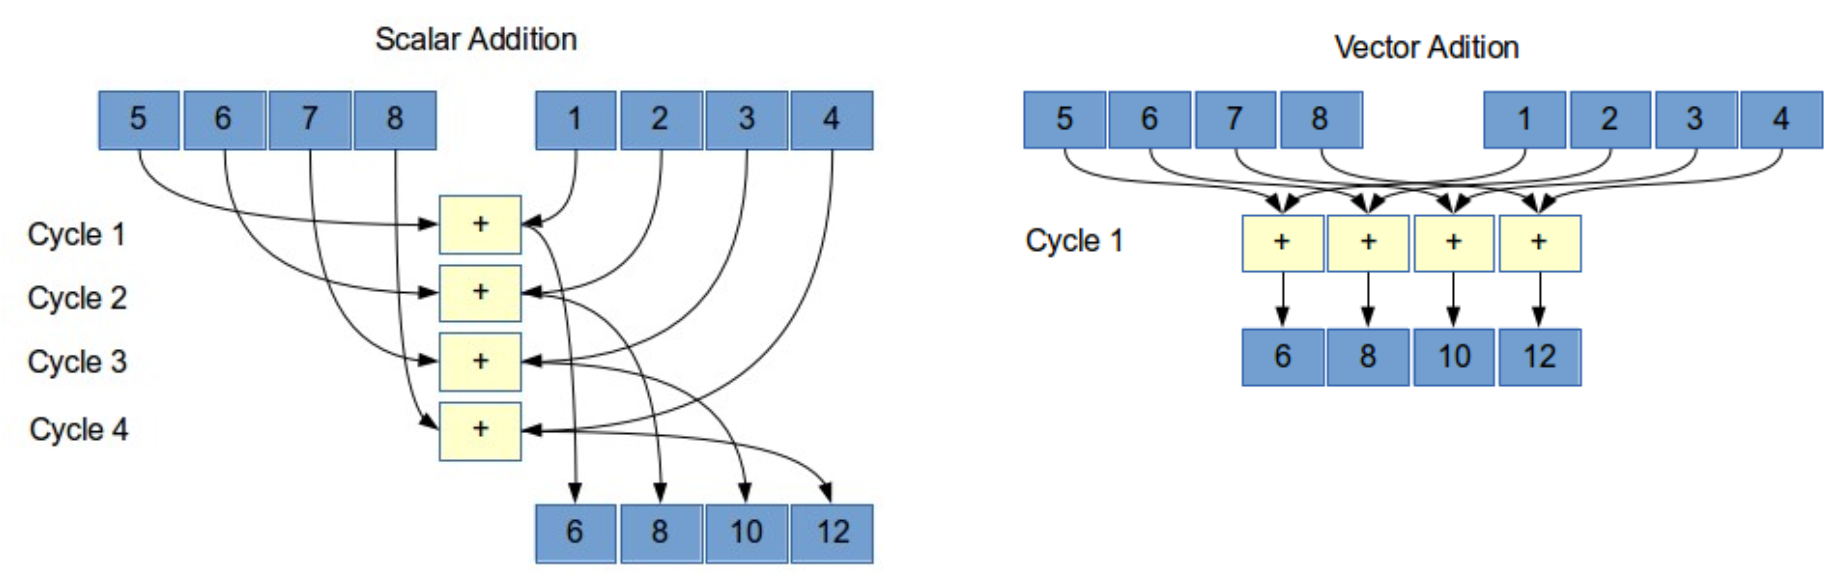
\includegraphics[width=\textwidth]{pictures/vectorization}
\end{frame}


%%%%%%%%%%%%%%%%%%%%%%%%%%%%%%%%%%%%%%%%%%%%%%%%%%%%%%%%%%%%%%%%%%%%%%%%%
\begin{frame}[fragile]{Vectorization Example}

For example consider this C program:
\begin{lstlisting}[language=C]
int a[8]; int b[8];
for (i=0; i < 8; i++)
    a[i] = a[i] + b[i];
\end{lstlisting}

Using the GCC vector extension\textsuperscript{*} we can rewrite this:
\begin{lstlisting}[language=C]
// using 256bit AVX2 register
typedef int vec8 __attribute__ ((vector_size (32)));
vec8 a, b;
a = a + b;
\end{lstlisting}

{\footnotesize *) Also supported by LLVM}
\end{frame}

%%%%%%%%%%%%%%%%%%%%%%%%%%%%%%%%%%%%%%%%%%%%%%%%%%%%%%%%%%%%%%%%%%%%%%%%%
\begin{frame}[fragile]{Auto-Vectorization}
\begin{itemize}
  \item Since there are many target specific ways of working with vectors, the compiler should take care of this
        for the programmer.
  \item The LLVM compiler has two vectorizers:
  \begin{itemize}
    \item Loop Vectorizer, which operates on Loops
    \item SLP Vectorizer, which merges scalars into vectors
  \end{itemize}
\end{itemize}
The LLVM IR supports vector data types natively:
\begin{lstlisting}[language=LLVM]
%vec1 = load <8 x i32>* %addr1
%vec2 = load <8 x i32>* %addr2
%vec3 = fmul <8 x i32> %vec1, %vec2
\end{lstlisting}
\end{frame}

%%%%%%%%%%%%%%%%%%%%%%%%%%%%%%%%%%%%%%%%%%%%%%%%%%%%%%%%%%%%%%%%%%%%%%%%%
\begin{frame}{Challenges}
\begin{itemize}
  \item The data we want to work on must be in a certain format
  \begin{itemize}
    \item It must fit into the vector registers of the CPU.
    \item The data must be correctly laid out for the SIMD instructions.
  \end{itemize}
  \item The program behaviour must be preserved, to this end the compiler guarantees:
  \begin{itemize}
    \item Data dependencies must be respected.
    \item The precision of the data types must be preserved, otherwise results become less precise.
  \end{itemize}
\end{itemize}
\end{frame}

%%%%%%%%%%%%%%%%%%%%%%%%%%%%%%%%%%%%%%%%%%%%%%%%%%%%%%%%%%%%%%%%%%%%%%%%%

\begin{frame}{Data Dependencies}
There are three types of data dependencies:
\begin{description}
  \item[Flow dependency]  An instruction depends on the result of a previous instruction (read-after-write), 
                          e.g.\ A = 5; B = A + 1;
  \item[Anti-dependency]  An instruction requires a value that is later updated (write-after-read),
                          e.g.\ A = 5; B = A + 1; A = 1;
  \item[Output dependency] Ordering of instructions will affect the final output value of a variable,
                           e.g.\ A = 5; A = 1;
\end{description}
The last two dependencies can be removed by using unique variable names.
\end{frame}

\subsection{Loop Vectorization}

%%%%%%%%%%%%%%%%%%%%%%%%%%%%%%%%%%%%%%%%%%%%%%%%%%%%%%%%%%%%%%%%%%%%%%%%%
\begin{frame}{}
\begin{itemize}
  \item The Loop Vectorizer rewrites loops to reduce the number of total operations.
  \item The idea is to "widen" instructions in loops to operate on multiple consecutive iterations.
  \item Optimizes the inner most loop.
\end{itemize}
\end{frame}


%%%%%%%%%%%%%%%%%%%%%%%%%%%%%%%%%%%%%%%%%%%%%%%%%%%%%%%%%%%%%%%%%%%%%%%%%

\begin{frame}[fragile]{Example}

\begin{itemize}
  \item Let's consider the previous C loop, but now with 1024 entries.
  \item Each 256 bit vector register can contain $256/32 = 8$ integers with 32 bits.
  \begin{itemize}
    \item We can convert the loop into one with $512 / 8 = 64$ iterations.
  \end{itemize}
\end{itemize}

\begin{lstlisting}[language=C]
int a[512]; int b[512];
for (i=0; i < 512; i += 8)
    a[i:i+7] = a[i:i+7] + b[i:i+7];
\end{lstlisting}
\end{frame}

%%%%%%%%%%%%%%%%%%%%%%%%%%%%%%%%%%%%%%%%%%%%%%%%%%%%%%%%%%%%%%%%%%%%%%%%%

\subsection{Superword Level Parallelismn}

\begin{frame}{}
\begin{itemize}
  \item Can exploit possible parallelism of inline code in a code block.
  \item Combine similar independent instructions into vector operations.
  \item Can unroll loops and optimize the inline code.
  \item Uses the control flow graph and looks into basic blocks for instructions to combine.
\end{itemize}
\end{frame}


%%%%%%%%%%%%%%%%%%%%%%%%%%%%%%%%%%%%%%%%%%%%%%%%%%%%%%%%%%%%%%%%%%%%%%%%%

\begin{frame}{Example}
The following statements are contained in the same block and are structurally the identical
(isomorphic). They are then parallized by a technique called \textit{statement packing}. 
\begin{center}
    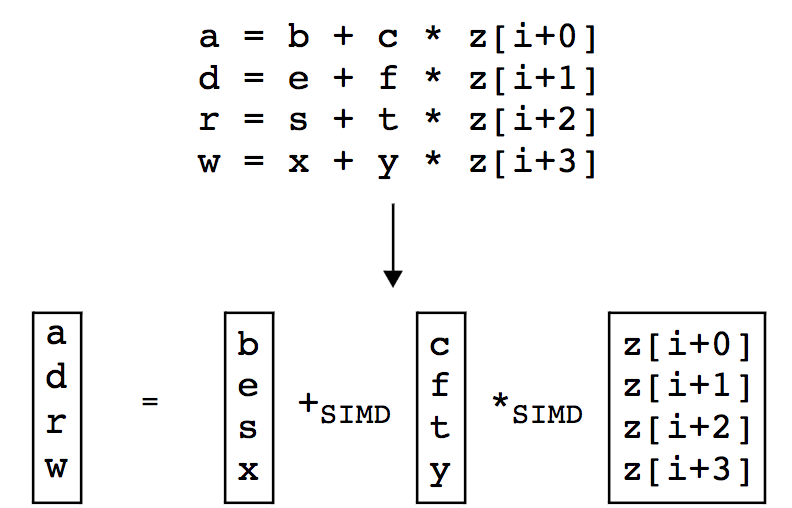
\includegraphics[width=.8\textwidth]{pictures/slp_example}
\end{center}
\end{frame}

%%%%%%%%%%%%%%%%%%%%%%%%%%%%%%%%%%%%%%%%%%%%%%%%%%%%%%%%%%%%%%%%%%%%%%%%%

\begin{frame}{SLP Vectorizer Steps}
\begin{itemize}
  \item As previously stated it uses the codes basic blocks to look for scalar instructions to combine.
  \item The Vectorizers processes the code from the bottom-up
  \item The SLP vectorizers uses the following stages
\begin{enumerate}
  \item Identify potential instruction patterns to vectorize
  \item Determine if it is profitable to vectorize the code
  \item Vectorize the code
\end{enumerate}
\end{itemize}
\end{frame}

%%%%%%%%%%%%%%%%%%%%%%%%%%%%%%%%%%%%%%%%%%%%%%%%%%%%%%%%%%%%%%%%%%%%%%%%%

\section{Summary}
\begin{frame}{Summary}
\begin{itemize}
  \item Code Generation
  \begin{itemize}
    \item The code generation process optimizes code for the target platform.
    \item Can replace unsupported operations and data types.
    \item Allows compiler frontends to avoid having to deal with target specific constraints.
  \end{itemize}

  \item Auto Vectorization
  \begin{itemize}
    \item Promises speedups for a lot of multimedia computations.
    \item The compiler frontend doesn't need to support vector types on it's own.
    \item Can optimize reasonably complex loops including control flow.
    \item Can greatly improve the energy efficency.
  \end{itemize}
\end{itemize}
\end{frame}

%%%%%%%%%%%%%%%%%%%%%%%%%%%%%%%%%%%%%%%%%%%%%%%%%%%%%%%%%%%%%%%%%%%%%%%%%

\begin{frame}{Reference}
\begin{itemize}
  \item The LLVM documentation \url{http://llvm.org/docs/}
  \item S.\ Larsen and S.\ Amarasinghe. Exploiting Superword Level Parallelism with Multimedia Instruction Sets. 
        In Proceedings of the SIGPLAN '00 Conference on Programming Language Design and Implementation, 
        Vancouver, B.C., June 2000
  \item M.\ Pandey and S.\ Sarda. LLVM Cookbook. Packt Publishing, May 2015
  \item Eli Bendersky. A deeper look into the LLVM code generator, 
        Article online \url{http://eli.thegreenplace.net/2013/02/25/a-deeper-look-into-the-llvm-code-generator-part-1}
\end{itemize}
\end{frame}

%%
%% the final slide (contact information) is generated automatically (at end document)
%%

\end{document}


%%%%%%%%%%%%%%%%%%%%%%%%%%%%%%%%%%%%%%%%%%%%%%%%%%%%%%%%%%%%%%%%%%%%%%%%%%%%%%%%%%%%%%%%%%%%%%%%%%%%%%%%%%%%%%%%%%%%%%%%%%%%%%%%%%%%%%%%%%%%%%%%
%%%%%%%%%%%%%%%%%%%%%%%%%%%%%%%%%%%%%%%%%%%%%%%%%%%%%%%%%%%%%%%%%%%%%%%%%%%%%%%%%%%%%%%%%%%%%%%%%%%%%%%%%%%%%%%%%%%%%%%%%%%%%%%%%%%%%%%%%%%%%%%%